\documentclass[12pt, letterpaper]{article}
\usepackage{amsmath}
\usepackage{amssymb}
\usepackage{graphicx} 
\title{STA 630 - Homework 1}
\author{Anthony Bernardi}
\date{January 31, 2025}
\begin{document}
\maketitle

\section{Problem 1 - Hoff 2.3}

\subsection{Part A}

Let X, Y, Z be random variables with joint density $p(x, y, z)$ which is proportional to $f(x, z) g(y, z) h(z)$. 

Show the following. 

\begin{equation} 
p(x | y, z) \propto f(x, z) 
\end{equation} 

We will do this with the definition of conditional probability. 

\begin{equation}
p(x | y, z) = \frac{p(x, y, z)}{p(y, z)} 
\end{equation} 

We can now re-write this in the following way. 

\begin{equation} 
\frac{p(x, y, z)}{p(y, z)} \propto f(x, z)
\end{equation}

We can continue re-writing to get something more workable. 

\begin{equation}
\frac{f(x, z) g(y, z) h(z)}{p(y , z)} \propto f(x, z) 
\end{equation} 

We can now continue to re-write until the cancellation becomes apparent. 

\begin{equation} 
\frac{f(x, z) g(y, z) h(z)}{g(y, z) h(z)} \propto f(x, z) 
\end{equation} 

We can now see that the g(y, z) and h(z) terms cancel out, and the final result is apparent. 

\begin{equation} 
p(x | y, z)  = f(x, z) \propto f(x, z) 
\end{equation} 

\subsection{Part B} 

Show the following. 

\begin{equation}
p(y | x, z) \propto g(y, z) 
\end{equation} 

We can do this in a similar way to part A, relying on the definition of conditional probability. 

\begin{equation} 
p(y | x, z) = \frac{p(x, y, z)}{p(x, z)} 
\end{equation} 

We'll now re-write. 

\begin{equation} 
\frac{p(x, y, z)}{p(x, z)} \propto g(y, z) 
\end{equation} 

Again, we can re-write to make the cancellation more apparent. 

\begin{equation} 
\frac{f(x, z) g(y, z) h(z)}{p(x, z)} \propto g(y, z)
\end{equation} 

Our final step and the cancellation becomes clear. 

\begin{equation} 
\frac{f(x, z) g(y, z) h(z)}{f(x, z) h(z)} \propto g(y, z) 
\end{equation} 

This cancels to reveal the following. 

\begin{equation} 
p(y | x, z) = g(y, z) \propto g(y, z) 
\end{equation} 

\subsection{Part C} 



\section{Problem 2}

Suppose that 6 observations are taken at random from a uniform distribution on the interval $(\theta - .5 , \theta + .5)$, with $\theta$ unknown, and we observe the following values. $(11.0, 11.5, 11.7, 11.1, 11.4, 10.9)$. 

Suppose the prior distribution of $\theta$ is uniform on the interval $(10, 20)$.

Derive the posterior of $\theta$. 

We will do this by first finding the likelihood function, and then multiplying this by the prior to derive our posterior function. 

The likelihood function is given by the following. 

\begin{equation}
L(\theta) = \prod_{i=1}^{6} \frac{1}{\theta + .5 - \theta + .5} = \frac{1}{(\theta + .5)^6 - (\theta - .5)^6} 
\end{equation} 

The prior is given by the following. 

\begin{equation} 
p(\theta) = \frac{1}{20 - 10} = \frac{1}{10} 
\end{equation} 

The posterior is given by the following. 

\begin{equation} 
p(\theta | x) \propto L(\theta) p(\theta) 
\end{equation} 

We can now plug in our likelihood and prior to get the following. 

\begin{equation}
p(\theta | x) \propto \frac{1}{(\theta + .5)^6 - (\theta - .5)^6} \frac{1}{10} 
\end{equation} 

We can now simplify this to get the following. 

\begin{equation} 
p(\theta | x) \propto \frac{1}{10((\theta + .5)^6 - (\theta - .5)^6)} 
\end{equation} 

If we want to get more specific, we can say the following regarding the distribution of the posterior. 

\begin{equation} 
p(\theta | x) \sim Uniform(10 * ((\theta + .5) - (\theta - .5)^6))
\end{equation} 

\section{Problem 3}

Suppose we are going to sample 100 individuals from a larger population, and we are asking if each individual person if they support policy Z or not. Let $Y_i = 1$ if they support the policy and $Y_i = 0$ if they do not. 

\subsection{Part a}

Assume $Y_1, Y_2, ..., Y_{100}$ are independent and identically distributed with $Y_i \sim Bernoulli(\theta)$, where $\theta$ is the proportion of the population that supports the policy. 

Write down the joint distribution of $P(Y_1 = y1, Y_2 = y2, ..., Y_{100} = y100 | \theta)$ in a compact form. Also, write down the form of $P(\sum Y_i = y | \theta)$. 

We can write the joint distribution in the following way, given the Bernoulli distribution. 

Given that we are looking for an exact value for each of the 100 individuals, we can write the joint distribution as the following. 

\begin{equation}
P(Y_1 = y1, Y_2 = y2, ..., Y_{100} = y100 | \theta) = \prod_{i=1}^{100} \theta^{y_i} (1 - \theta)^{1 - y_i} 
\end{equation} 

We will now handle the sum, which we can think about as the sum of the Bernoulli random variables, which is a binomial distribution. 

\begin{equation} 
P(\sum Y_i = y | \theta) = \binom{100}{y} \theta^y (1 - \theta)^{100 - y} 
\end{equation} 

\subsection{Part b} 

For a moment, suppose you believed that the parameter $\theta$ had the following characteristic. $\theta \in \{0, 0.1, \dots , 0.9, 1.0}$. 

Given that the results of the survey were $\sum_{i=1}^100 Y_i = 57$, compute $P(\sum Y_i = 57 | \theta)$ for each of these 11 values and plot these probabilities as a function of $theta$. 

Given this information, we can use the Binomial distribution for each possible parameter value in the parameter space, and plot the outputs of these probabilities with R. 

The following code was used to generate the values, and the plot is attached. 

\begin{verbatim}
theta_v <- seq(0, 1, by = 0.1) 

# fixed values 
x <- 57 
n < 100 
likelihoods <- vector(length = 11) 

for (param in theta_v){
  i = 0 
  likelihoods[i] <- dbinom(x, n, param) 
  i = i + 1 
}

plot(x = theta_v , 
     y = likelihoods, 
     type = "l", 
     xlab = "Theta", 
     ylab = "P(Y = 57 | Theta)", 
     main = "Probability of Y = 57 for different values of Theta")
\end{verbatim}

\begin{figure}
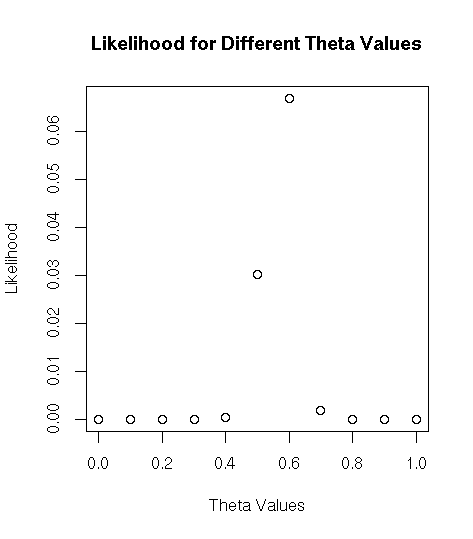
\includegraphics{/home/adbucks/Documents/sta_630/Likelihood_plot_3.1b.png}
\end{figure}

\subsection{Part c} 





































\end{document}
